So far we have discussed and implemented methods for the space-homogeneous kinetic and particle models, as well as the particle model with the space variable included. The particle model simulation has shown to closely reflect the behaviour predicted by the analysis, and is a good approximation to the kinetic model when the number of particles is high enough. It is also very efficient, many particles can be simulated very quickly. However, when spatial heterogeneity is introduced, complexity will increase hugely as the function $phi$ must be evaluated $N-1$ times for each of the $N$ particles. In the kinetic model, $\phi$ appears only within the integral, which will be easier to numerically approximate. Therefore at this stage it is unwise to compare the two methods solely on computational speed. The next step in this direction is to include various choices of $\phi$ that do not satisfy the restrictions required for the analysis \eqref{eq:phi}, to see if this has any effect on the convergence of the system. 

Also, the error in the homogeneous kinetic approximation has not been rigorously checked. Theoretically the approximations will be first order in time and space, ideally one would have numeric confirmation of this. To this end, a higher order scheme will be implemented for the advection term in the finite difference method such as the third-order upwind scheme. Similarly, an implicit method used in the finite volume approach would be a simple way to increase accuracy. For example, a Crank-Nicolson scheme could be applied to the diffusive term. Finite volume methods provide many ways in which to solve the advection term whilst conserving mass, here we have only begun the exploration. The Lax-Wendroff scheme is second order in space and time, and would bring the truncation error of the advective term in line with that of the diffusion term. The change of variables described in Section\ref{sec:hominvmeas} could also be utilised to assess the accuracy of the scheme. It gives another way of approximating the homogeneous system, only requiring the simulation of the Ornstein-Uhlenbeck process and the time integral of the herding function.

As well as consolidating the method for the space-homogeneous case, the method should be extended to solve the two-dimensional space-heterogeneous case. The one-dimensional finite volume scheme is the ideal base for this. This would allow us to ask and answer questions that the analysis cannot. For example, are their any combinations of interaction functions $\phi$ and initial distributions that mean the particle system will not homogenise in space? This would be in stark contrast to the behaviour of the kinetic model, and would suggest the existence of another invariant measure. We conjecture that a compactly supported interaction function, and an initial distribution in which two clusters of particles are placed diametrically opposite each other may produce such a measure. Figure \ref{fig:compactphi} shows such a configuration.

\begin{figure}
    \centering
    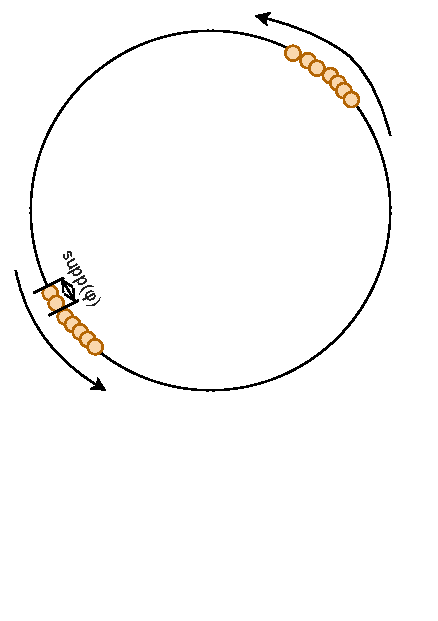
\includegraphics[width=0.5\linewidth, trim={0 3cm 0 0}, clip]{Figures/compactphi}
    \caption[A Potential Initial Configuration]{A possible inital configuration that may cause spatial heterogeneity.}
    \label{fig:compactphi}
\end{figure}

\subsection{Application to Biological Systems}
As already discussed, many systems in nature can be thought of as interacting particles. There is a possibility this model may be used to describe biological phenomena such as the movement of \emph{Schistocerca gregaria}, desert locusts seen in 
